\documentclass[compress]{beamer}

\usepackage{beamerthemesplit}

% language
\usepackage[american]{babel}
\usepackage[utf8x]{inputenc}

\usepackage{ucs}
\usepackage{graphicx}
\usepackage{multirow}

% bib
\bibliographystyle{alphaurl}

% TikZ
\usepackage{tikz}

% beamer
\usetheme{Frankfurt}
\usecolortheme{default}
\usepackage{appendixnumberbeamer}

%
% SPECIAL IMPORTS
%
\usepackage{xparse}
\usepackage{boxedminipage}


%
% GENERAL
%

% environments
\NewDocumentEnvironment{JWboxed}{mm}%
  {\begin{figure}[ht]%
   \small%
   \begin{boxedminipage}{\linewidth}%
  }%
  {\end{boxedminipage}%
   \caption{#1}%
   \label{#2}%
   \end{figure}%
  }

% functionality
\newenvironment{JWfunc}[3]%
{\begin{JWboxed}{#2}{#3}%
 \begin{center}\textbf{{Functionality #1}}\end{center}%
}%
{\end{JWboxed}}

\newenvironment{JWfuncSteps}[0]{\begin{itemize}}{\end{itemize}}

\newcommand{\JWfuncSym}[2]{$\mathcal{F}^\mathrm{#1}_\mathrm{#2}$}

%protocol
\newenvironment{JWprotocol}[3]%
{\begin{JWboxed}{#2}{#3}%
 \begin{center}\textbf{{Protocol #1}}\end{center}%
}%
{\end{JWboxed}}

\newenvironment{JWprotoSteps}[0]{\begin{enumerate}}{\end{enumerate}}

\newcommand{\JWprotoPhase}[1]{\paragraph{#1}}

\newcommand{\JWprotoSym}[2]{$\Pi^\mathrm{#1}_\mathrm{#2}$}

%misc
\newcommand{\JWbinary}[1]{\texttt{#1}}
\newcommand{\JWtodo}[1]{\fbox{TODO: #1}}
\newcommand{\JWmsgTT}[2]{(\texttt{#1}, \texttt{#2})}
\newcommand{\JWmsgT}[1]{(\texttt{#1})}
\newcommand{\JWmsgTP}[2]{(\texttt{#1}, #2)}
\newcommand{\JWpath}[1]{\texttt{#1}}

\DeclareDocumentCommand\JWdef{mmg}{%
  {\label{def:#2}\emph{#1\IfNoValueF{#3}{#3}}%
  } (#2%
  \IfNoValueF{#3}{#3}%
  )%
}

\newenvironment{JWtodoBox}[0]%
  {\begin{boxedminipage}{\linewidth}TODO:\par}{\end{boxedminipage}}

%chapters
\makeatletter
\newcommand{\JWlone}{\@ifstar
  \JWloneNoTOC%
  \JWloneTOC%
}
\newcommand{\JWltwo}{\@ifstar
  \JWltwoNoTOC%
  \JWltwoTOC%
}
\newcommand{\JWlthree}{\@ifstar
  \JWlthreeNoTOC%
  \JWlthreeTOC%
}
\newcommand{\JWlfour}{\@ifstar
  \JWlfourNoTOC%
  \JWlfourTOC%
}
\newcommand{\JWlfive}{\@ifstar
  \JWlfiveNoTOC%
  \JWlfiveTOC%
}
\newcommand{\JWlsix}{\@ifstar
  \JWlsixNoTOC%
  \JWlsixTOC%
}

\newcommand{\JWloneTOC}[1]{\chapter{#1}}
\newcommand{\JWloneNoTOC}[1]{\chapter*{#1}}
\newcommand{\JWltwoTOC}[1]{\section{#1}}
\newcommand{\JWltwoNoTOC}[1]{\section*{#1}}
\newcommand{\JWlthreeTOC}[1]{\subsection{#1}}
\newcommand{\JWlthreeNoTOC}[1]{\subsection*{#1}}
\newcommand{\JWlfourTOC}[1]{\subsubsection{#1}}
\newcommand{\JWlfourNoTOC}[1]{\subsubsection*{#1}}
\newcommand{\JWlfiveTOC}[1]{\paragraph{#1}}
\newcommand{\JWlfiveNoTOC}[1]{\paragraph*{#1}}
\newcommand{\JWlsixTOC}[1]{\subparagraph{#1}}
\newcommand{\JWlsixNoTOC}[1]{\subparagraph*{#1}}

%links and names
\newcommand{\JWnamedlink}[2]{\href{#1}{#2}}
\newcommand{\JWurl}[1]{\href{#1}{#1}}

%code/commands
\newcommand{\JWcode}[1]{\texttt{#1}}
\newcommand{\JWcmd}[1]{\texttt{\$ #1}}
\newcommand{\JWhsExt}[1]{\texttt{#1}}


%lemmata/theorems
\newtheorem{thm}{Theorem}
\newtheorem{lem}[thm]{Lemma}


%
% SPECIALIZED SHORTCUTS
%
\newcommand{\JWprotoSymOPE}[0]{\JWprotoSym{}{OPE}}
\newcommand{\JWfuncSymOPE}[0]{\JWfuncSym{(k, n)}{OPE}}
\newcommand{\JWfuncSymOPEnp}[0]{\JWfuncSym{}{OPE}}
\newcommand{\JWfuncSymOAFE}[0]{\JWfuncSym{seq-ot}{OAFE}}
\newcommand{\JWfieldGeneral}[0]{\mathbb{F}_{2^k}}
\newcommand{\JWadv}[0]{$\mathcal{A}$}
\newcommand{\JWpOne}[0]{Goliath}
\newcommand{\JWpTwo}[0]{David}
\newcommand{\JWtoken}[0]{Token}
\newcommand{\JWnegl}[0]{\text{*) Except for a negligible probability.}}
\newcommand{\JWtitle}[0]{Efficient Secure Function Evaluation using Garbled %
Arithmetic Circuits and Untrusted Tamper--Proof Hardware}
\newcommand{\entspricht}{\stackrel{\scriptscriptstyle\wedge}{=}}

%tools ans versions
\newcommand{\JWThaskell}[0]{Haskell}
\newcommand{\JWTghc}[0]{GHC}
\newcommand{\JWTXghc}[0]{Glasgow Haskell Compiler}
\newcommand{\JWTLhaskell}[0]{\JWnamedlink{http://haskell.org}{\JWThaskell}}
\newcommand{\JWTLhaddock}[0]{\JWnamedlink{http://www.haskell.org/haddock/}%
                            {Haddock}}
\newcommand{\JWTLcabal}[0]{\JWnamedlink{http://www.haskell.org/cabal/}%
                            {Cabal}}
\newcommand{\JWTXLghc}[0]{\JWnamedlink{http://www.haskell.org/ghc/}{\JWTXghc}}
\newcommand{\JWTVghc}{7.6.1}
\newcommand{\JWTntl}[0]{NTL}
\newcommand{\JWTLntl}[0]{\JWnamedlink{http://www.shoup.net/ntl/}{\JWTntl}}
\newcommand{\JWTcpp}[0]{C++}
\newcommand{\JWTc}[0]{C}
\newcommand{\JWTgit}[0]{git}
\newcommand{\JWTquickcheck}[0]{QuickCheck}
\newcommand{\JWTLhunit}[0]{\JWnamedlink{http://hunit.sourceforge.net/}{HUnit}}
\newcommand{\JWTLmonadcryptorandom}[0]%
  {\JWnamedlink{http://hackage.haskell.org/package/monadcryptorandom}%
  {\texttt{monadcryptorandom}}}
\newcommand{\JWTLhaskellForMaths}[0]%
  {\JWnamedlink{http://hackage.haskell.org/package/HaskellForMaths}%
  {\texttt{HaskellForMaths}}}
\newcommand{\JWTLdrbg}[0]%
  {\JWnamedlink{http://hackage.haskell.org/package/DRBG}{\texttt{DRBG}}}
\newcommand{\JWTXprotobuf}{Google\TTra{} Protocol Buffers}
\newcommand{\JWTprotobuf}{Protocol Buffers}
\newcommand{\JWTXLprotobuf}[0]%
  {\JWnamedlink{http://code.google.com/apis/protocolbuffers/}{\JWTXprotobuf{}}}
\newcommand{\JWTLhackage}[0]%
  {\JWnamedlink{http://hackage.haskell.org/packages/hackage.html}{HackageDB}}


%binaries
\newcommand{\JWBpOne}[0]{\JWbinary{\JWpOne{}}}
\newcommand{\JWBpTwo}[0]{\JWbinary{\JWpTwo{}}}
\newcommand{\JWBtoken}[0]{\JWbinary{\JWtoken{}}}

%misc
\newcommand{\JWport}[1]{\texttt{#1}}
\def\TReg{\textsuperscript{\textregistered}}
\def\TCop{\textsuperscript{\textcopyright}}
\def\TTra{\textsuperscript{\texttrademark}}


\title{\JWtitle{}}

\author{Johannes Weiß}

\date{Januar 2013}

\begin{document}

\frame{\titlepage}

%
% OUTLINE
%
\section{Outline}

\subsection{Outline}

\frame {

  \frametitle{Outline}

  \begin{itemize}

    \item What is the Problem?

    \item Oblivious Affine Function Evaluation (OAFE)

    \item Secure Arithmetic

    \item Main Results

    \item Implementation

    \item Evaluation

  \end{itemize}

}


%
% WHAT IS THE PROBLEM
%

\section{Problem}

% WHAT IS THE PROBLEM
\subsection{What is the Problem?}

\frame {

  \frametitle{What is the Problem?}

  \begin{itemize}

    \item Secure Function Evaluation (SFE)

    \item Oblivious Polynomial Evaluation (OPE)

  \end{itemize}

}

% OTHER APPROACHES
\subsection{Other Approaches}

\frame {

  \frametitle{Other Approaches}

  Classic:
  \begin{itemize}

    \item Yao's \JWdefn{Garbled Circuit}{GC} \cite{yao86} approach

  \end{itemize}

  Promising:
  \begin{itemize}

    \item \emph{Efficient Multi--Party Computation Over Rings} \cite{cramer03},
      based on \emph{Simulation of Formulas by Bounded--Width Programs}
      \cite{cleve91}

    \item Garbled Arithmetic Circuits \cite{gac2012}

  \end{itemize}

  Problems:
  \begin{itemize}

    \item No Square \& Multiply

    \item Polynomial Time Complexity

  \end{itemize}

}

% INITIAL IDEA
\subsection{Initial Idea}

\frame {

  \frametitle{Initial Idea}

  Initial idea:

  \begin{itemize}

    \item Goal: Efficient SFE (arbitrary arithmetic circuits)

    \item Methodology: Bridging the ideas of some papers

    \item Main Focus: Implementation

  \end{itemize}

}

% OPE
\subsection{OPE}

\frame {

  \frametitle{Goal: Oblivious Polynomial Evaluation (OPE)}

  \begin{align*}
    %
    y = f(x) = \sum_{i=0}^n a_ix^i
    %
  \end{align*}

  \begin{figure}[h!]
    \centering

    \begin{tikzpicture}[>=stealth]

      \node (OPE) at (8.5,0) {OPE};
      \draw (OPE) +(-1.5,-1.15) rectangle +(1.5,0.65);

      \draw [<-] (OPE) ++(-1.5,0.25) node [anchor=west] {} -- +(-0.75,0) node
      [anchor=east] {$\JWfieldGeneral^{n+1} \ni a$};

      \draw [<-] (OPE) ++(1.5,0.25) node [anchor=east] {} -- +(0.75,0) node
      [anchor=west] {$x \in \JWfieldGeneral$};

      \draw [->] (OPE) ++(1.5,-0.75) node [anchor=east] {$\sum_{i=0}^n a_ix^i$}
      -- +(0.75,0)
      node [anchor=west] {$y \in \JWfieldGeneral$};

    \end{tikzpicture}
  \end{figure}

  \begin{itemize}

    \item First party chooses polynomial, learns nothing

    \item Second Party chooses node $x$ and learns $y = f(x)$

  \end{itemize}
}


%
% OAFE
%

\section{OAFE}

\subsection{OAFE}

\frame {

  \frametitle{Basis: Oblivious Affine Function Evaluation (OAFE)}

  Main building block: OAFE \cite{davidgoliath}.

  \begin{figure}[h!]
    \centering

    \begin{tikzpicture}[>=stealth]
      \node (OAFE) at (8.5,0) {OAFE};
      \draw (OAFE) +(-1.5,-1.15) rectangle +(1.5,0.65);
      \draw [<-] (OAFE) ++(-1.5,0.25) node [anchor=west] {} -- +(-0.75,0) node
      [anchor=east] {$a$};
      \draw [<-] (OAFE) ++(-1.5,-0.25) node [anchor=west] {} -- +(-0.75,0) node
      [anchor=east] {$b$};
      \draw [<-] (OAFE) ++(1.5,0.25) node [anchor=east] {} -- +(0.75,0) node
      [anchor=west] {$x$};
      \draw [->] (OAFE) ++(1.5,-0.75) node [anchor=east] {$ax+b$} -- +(0.75,0)
      node [anchor=west] {$y$};
      %
    \end{tikzpicture}
  \end{figure}
}


%
% SECURE ARITHMETIC
%

\section{Secure Arithmetic}

\subsection{Definition}

\frame {

  \frametitle{Secure Arithmetic}

  \begin{itemize}

    \item Goal: Secure and composable encoding of additions ($+$) and
      multiplications ($\cdot$)

    \item Optimally, support Square \& Multiply (arbitrary arithmetic circuits)

  \end{itemize}

  \begin{figure}
    \centering
    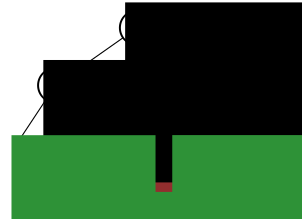
\includegraphics[width=6cm]{sample-polynomial-no-DRAE}
  \end{figure}

}

\frame {

  \frametitle{Dual Randomized Affine Value (DRAV)}

  \begin{figure}
    \centering
    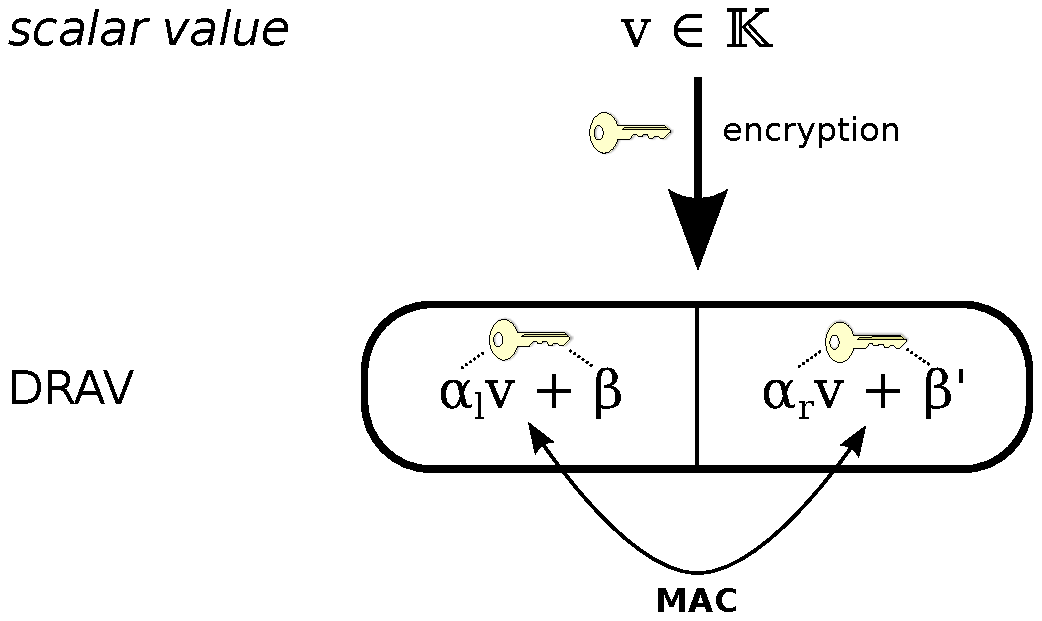
\includegraphics[width=\textwidth]{DRAV}
  \end{figure}

}

\subsection{Protocol Basics}

\frame {

  \frametitle{Protocol Basics}

  First Party (Goliath):

  \begin{enumerate}

    \item Defines function

    \item Sets up OAFE functionality (coefficients of the affine functions)

  \end{enumerate}

  Second Party (David):

  \begin{enumerate}

    \item Encrypts its input to a DRAV using the OAFE functionality

    \item Calculates (encrypted) intermediate results

      \begin{itemize}

        \item Performs calculations

        \item Evaluates OAFEs using intermediate DRAVs, obtaining new
          intermediate DRAVs

      \end{itemize}

    \item Decrypts the last DRAV (using OAFE)

  \end{enumerate}

}

% ADDITION
\subsection{Addition}

\frame {

  \frametitle{Addition}

  Addition of $\widetilde{a}$ and $\widetilde{b}$ performed component--wise.

  \begin{align*}
    %
    \widetilde{a} &=
    \begin{pmatrix}
      \alpha_l \cdot a + \beta_1\\
      \alpha_r \cdot a + \beta_2
    \end{pmatrix} &
    %
    \widetilde{b} &=
    \begin{pmatrix}
      \alpha_l \cdot b + \beta_3\\
      \alpha_r \cdot b + \beta_4
    \end{pmatrix}\\
    %
  \end{align*}

  \noindent{}Yielding $\widetilde{y} = \widetilde{a} + \widetilde{b}$

  \begin{align*}
    %
    \widetilde{y} &=
    \begin{pmatrix}
      \alpha_l \cdot a + \beta_1 + \alpha_l \cdot b + \beta_3\\
      \alpha_r \cdot a + \beta_2 + \alpha_r \cdot b + \beta_4\\
    \end{pmatrix} =
    \begin{pmatrix}
      \alpha_l \cdot (a+b) + (\beta_1 + \beta_3)\\
      \alpha_r \cdot (a+b) + (\beta_2 + \beta_4)\\
    \end{pmatrix}\\
    %
  \end{align*}

}

% MULTIPLICATION
\subsection{Multiplication}

\frame {

  \frametitle{Multiplication}

  \begin{align*}
    %
  \begin{pmatrix}\mathfrak{A}\\\mathfrak{G}\end{pmatrix} & =
  \begin{pmatrix}\alpha_l\\\alpha_r r_6\end{pmatrix} \cdot D_l(\widetilde{x}) +
  \begin{pmatrix}-r_1\\-r_7\end{pmatrix} &
    %
  \begin{pmatrix}\mathfrak{B}\\\mathfrak{H}\end{pmatrix} & =
  \begin{pmatrix}1\\r_5\end{pmatrix} \cdot D_l(\widetilde{y}) +
  \begin{pmatrix}-r_2\\r_8\end{pmatrix}\\
    %
  \begin{pmatrix}\mathfrak{E}\\\mathfrak{C}\end{pmatrix} & =
  \begin{pmatrix}\alpha_r\\\alpha_l r_2\end{pmatrix} \cdot D_r(\widetilde{x}) +
  \begin{pmatrix}-r_5\\r_3\end{pmatrix} &
    %
  \begin{pmatrix}\mathfrak{F}\\\mathfrak{D}\end{pmatrix} & =
  \begin{pmatrix}1\\r_1\end{pmatrix} \cdot D_r(\widetilde{y}) +
  \begin{pmatrix}-r_6\\r_4\end{pmatrix}\\
    %
  \end{align*}

  \noindent{}Calculation of the (encrypted) result:
  \begin{align*}
    \widetilde{z} & =
    \begin{pmatrix}
      \mathfrak{A} \cdot \mathfrak{B}+\mathfrak{C}+\mathfrak{D}\\
      \mathfrak{E} \cdot \mathfrak{F}+\mathfrak{G}+\mathfrak{H}
    \end{pmatrix}
    =
    \begin{pmatrix}
      \alpha_l xy + \beta\\
      \alpha_r xy + \beta'
    \end{pmatrix}
    \\
  \end{align*}

  \noindent{}$\widetilde{z}$'s encryption keys:
  \begin{align*}
    \beta & = r_1r_2 + r_3 + r_4 &
    \beta' & = r_5r_6 + r_7 + r_8 \\
    %
  \end{align*}
}

\frame {

  \frametitle{Problem \& Solution}

  Problem:

  \begin{itemize}

    \item Adversary learns the OAFE outputs $\mathfrak{A}$ to
      $\mathfrak{H}$.

    \item Security Proof too complicated (\emph{maybe impossible?})

  \end{itemize}

  Solution (\emph{Radicals Trick}):

  \begin{itemize}

    \item Split $\mathfrak{A}$ to $\mathfrak{H}$ in two linear functions
      (respectively)

    \item Secret Sharing

    \item Security proof easy

  \end{itemize}

}



%
% MAIN RESULTS
%

\section{Main Results}

\subsection{Main Results}

\frame {

  \frametitle{Main Results / Contribution}

  \begin{itemize}

    \item UC--secure \cite{canetti01} against all passive and active adversaries

    \item Linear time complexity (in the number of arithmetic operations)

    \item Working implementation

  \end{itemize}

}


%
% IMPLEMENTATION
%
\section{Implementation}

\subsection{Implementation}

\frame {

  \frametitle{Implementation}

  \begin{itemize}

    \item Implemented in the lazy, functional language Haskell

    \item Open--sourced at available
      \JWnamedlinkfn{https://github.com/weissi/diplomarbeit}{online}

  \end{itemize}

}


%
% EVALUATION
%

\section{Evaluation}

\subsection{Evaluation}

\frame {
  \frametitle{Evaluation}

  % Created by tikzDevice version 0.6.2-92-0ad2792 on 2013-01-17 18:11:30
% !TEX encoding = UTF-8 Unicode
\begin{tikzpicture}[x=1pt,y=1pt]
\definecolor[named]{fillColor}{rgb}{1.00,1.00,1.00}
\path[use as bounding box,fill=fillColor,fill opacity=0.00] (0,0) rectangle (325.21,216.81);
\begin{scope}
\path[clip] ( 49.20, 61.20) rectangle (300.01,167.61);
\definecolor[named]{drawColor}{rgb}{1.00,0.00,0.00}

\path[draw=drawColor,line width= 0.4pt,line join=round,line cap=round] ( 58.49, 68.60) --
	( 70.71, 72.38) --
	( 82.94, 76.15) --
	( 95.16, 79.72) --
	(107.38, 83.08) --
	(119.60, 86.63) --
	(131.83, 90.36) --
	(144.05, 93.81) --
	(156.27, 97.50) --
	(168.50,101.18) --
	(180.72,104.83) --
	(192.94,108.49) --
	(205.16,112.24) --
	(217.39,115.69) --
	(229.61,119.67) --
	(241.83,123.29) --
	(254.06,127.25) --
	(266.28,130.99) --
	(278.50,135.15) --
	(290.73,138.83);

\path[draw=drawColor,line width= 0.4pt,line join=round,line cap=round] ( 58.49, 68.60) circle (  2.25);

\path[draw=drawColor,line width= 0.4pt,line join=round,line cap=round] ( 70.71, 72.38) circle (  2.25);

\path[draw=drawColor,line width= 0.4pt,line join=round,line cap=round] ( 82.94, 76.15) circle (  2.25);

\path[draw=drawColor,line width= 0.4pt,line join=round,line cap=round] ( 95.16, 79.72) circle (  2.25);

\path[draw=drawColor,line width= 0.4pt,line join=round,line cap=round] (107.38, 83.08) circle (  2.25);

\path[draw=drawColor,line width= 0.4pt,line join=round,line cap=round] (119.60, 86.63) circle (  2.25);

\path[draw=drawColor,line width= 0.4pt,line join=round,line cap=round] (131.83, 90.36) circle (  2.25);

\path[draw=drawColor,line width= 0.4pt,line join=round,line cap=round] (144.05, 93.81) circle (  2.25);

\path[draw=drawColor,line width= 0.4pt,line join=round,line cap=round] (156.27, 97.50) circle (  2.25);

\path[draw=drawColor,line width= 0.4pt,line join=round,line cap=round] (168.50,101.18) circle (  2.25);

\path[draw=drawColor,line width= 0.4pt,line join=round,line cap=round] (180.72,104.83) circle (  2.25);

\path[draw=drawColor,line width= 0.4pt,line join=round,line cap=round] (192.94,108.49) circle (  2.25);

\path[draw=drawColor,line width= 0.4pt,line join=round,line cap=round] (205.16,112.24) circle (  2.25);

\path[draw=drawColor,line width= 0.4pt,line join=round,line cap=round] (217.39,115.69) circle (  2.25);

\path[draw=drawColor,line width= 0.4pt,line join=round,line cap=round] (229.61,119.67) circle (  2.25);

\path[draw=drawColor,line width= 0.4pt,line join=round,line cap=round] (241.83,123.29) circle (  2.25);

\path[draw=drawColor,line width= 0.4pt,line join=round,line cap=round] (254.06,127.25) circle (  2.25);

\path[draw=drawColor,line width= 0.4pt,line join=round,line cap=round] (266.28,130.99) circle (  2.25);

\path[draw=drawColor,line width= 0.4pt,line join=round,line cap=round] (278.50,135.15) circle (  2.25);

\path[draw=drawColor,line width= 0.4pt,line join=round,line cap=round] (290.73,138.83) circle (  2.25);
\end{scope}
\begin{scope}
\path[clip] (  0.00,  0.00) rectangle (325.21,216.81);
\definecolor[named]{drawColor}{rgb}{0.00,0.00,0.00}

\path[draw=drawColor,line width= 0.4pt,line join=round,line cap=round] ( 95.16, 61.20) -- (290.73, 61.20);

\path[draw=drawColor,line width= 0.4pt,line join=round,line cap=round] ( 95.16, 61.20) -- ( 95.16, 55.20);

\path[draw=drawColor,line width= 0.4pt,line join=round,line cap=round] (144.05, 61.20) -- (144.05, 55.20);

\path[draw=drawColor,line width= 0.4pt,line join=round,line cap=round] (192.94, 61.20) -- (192.94, 55.20);

\path[draw=drawColor,line width= 0.4pt,line join=round,line cap=round] (241.83, 61.20) -- (241.83, 55.20);

\path[draw=drawColor,line width= 0.4pt,line join=round,line cap=round] (290.73, 61.20) -- (290.73, 55.20);

\node[text=drawColor,anchor=base,inner sep=0pt, outer sep=0pt, scale=  1.00] at ( 95.16, 39.60) {2000};

\node[text=drawColor,anchor=base,inner sep=0pt, outer sep=0pt, scale=  1.00] at (144.05, 39.60) {4000};

\node[text=drawColor,anchor=base,inner sep=0pt, outer sep=0pt, scale=  1.00] at (192.94, 39.60) {6000};

\node[text=drawColor,anchor=base,inner sep=0pt, outer sep=0pt, scale=  1.00] at (241.83, 39.60) {8000};

\node[text=drawColor,anchor=base,inner sep=0pt, outer sep=0pt, scale=  1.00] at (290.73, 39.60) {10000};

\path[draw=drawColor,line width= 0.4pt,line join=round,line cap=round] ( 49.20, 65.14) -- ( 49.20,163.67);

\path[draw=drawColor,line width= 0.4pt,line join=round,line cap=round] ( 49.20, 65.14) -- ( 43.20, 65.14);

\path[draw=drawColor,line width= 0.4pt,line join=round,line cap=round] ( 49.20, 84.85) -- ( 43.20, 84.85);

\path[draw=drawColor,line width= 0.4pt,line join=round,line cap=round] ( 49.20,104.55) -- ( 43.20,104.55);

\path[draw=drawColor,line width= 0.4pt,line join=round,line cap=round] ( 49.20,124.26) -- ( 43.20,124.26);

\path[draw=drawColor,line width= 0.4pt,line join=round,line cap=round] ( 49.20,143.96) -- ( 43.20,143.96);

\path[draw=drawColor,line width= 0.4pt,line join=round,line cap=round] ( 49.20,163.67) -- ( 43.20,163.67);

\node[text=drawColor,rotate= 90.00,anchor=base,inner sep=0pt, outer sep=0pt, scale=  1.00] at ( 34.80, 65.14) {0};

\node[text=drawColor,rotate= 90.00,anchor=base,inner sep=0pt, outer sep=0pt, scale=  1.00] at ( 34.80, 84.85) {10};

\node[text=drawColor,rotate= 90.00,anchor=base,inner sep=0pt, outer sep=0pt, scale=  1.00] at ( 34.80,104.55) {20};

\node[text=drawColor,rotate= 90.00,anchor=base,inner sep=0pt, outer sep=0pt, scale=  1.00] at ( 34.80,124.26) {30};

\node[text=drawColor,rotate= 90.00,anchor=base,inner sep=0pt, outer sep=0pt, scale=  1.00] at ( 34.80,143.96) {40};

\node[text=drawColor,rotate= 90.00,anchor=base,inner sep=0pt, outer sep=0pt, scale=  1.00] at ( 34.80,163.67) {50};

\path[draw=drawColor,line width= 0.4pt,line join=round,line cap=round] ( 49.20, 61.20) --
	(300.01, 61.20) --
	(300.01,167.61) --
	( 49.20,167.61) --
	( 49.20, 61.20);
\end{scope}
\begin{scope}
\path[clip] (  0.00,  0.00) rectangle (325.21,216.81);
\definecolor[named]{drawColor}{rgb}{0.00,0.00,0.00}

\node[text=drawColor,anchor=base,inner sep=0pt, outer sep=0pt, scale=  1.00] at (174.61, 15.60) {Polynomial Degree};

\node[text=drawColor,rotate= 90.00,anchor=base,inner sep=0pt, outer sep=0pt, scale=  1.00] at ( 10.80,114.41) {Running Time [s]};
\end{scope}
\begin{scope}
\path[clip] ( 49.20, 61.20) rectangle (300.01,167.61);
\definecolor[named]{drawColor}{rgb}{0.00,1.00,0.00}

\path[draw=drawColor,line width= 0.4pt,dash pattern=on 1pt off 3pt ,line join=round,line cap=round] ( 58.49, 68.91) --
	( 70.71, 72.84) --
	( 82.94, 76.89) --
	( 95.16, 81.02) --
	(107.38, 85.24) --
	(119.60, 89.21) --
	(131.83, 93.11) --
	(144.05, 97.16) --
	(156.27,101.21) --
	(168.50,105.37) --
	(180.72,109.47) --
	(192.94,114.08) --
	(205.16,118.51) --
	(217.39,122.90) --
	(229.61,127.41) --
	(241.83,131.54) --
	(254.06,136.54) --
	(266.28,141.17) --
	(278.50,146.42) --
	(290.73,150.96);

\path[draw=drawColor,line width= 0.4pt,line join=round,line cap=round] ( 56.50, 66.92) rectangle ( 60.48, 70.91);

\path[draw=drawColor,line width= 0.4pt,line join=round,line cap=round] ( 68.72, 70.84) rectangle ( 72.71, 74.83);

\path[draw=drawColor,line width= 0.4pt,line join=round,line cap=round] ( 80.94, 74.89) rectangle ( 84.93, 78.88);

\path[draw=drawColor,line width= 0.4pt,line join=round,line cap=round] ( 93.16, 79.02) rectangle ( 97.15, 83.01);

\path[draw=drawColor,line width= 0.4pt,line join=round,line cap=round] (105.39, 83.24) rectangle (109.38, 87.23);

\path[draw=drawColor,line width= 0.4pt,line join=round,line cap=round] (117.61, 87.22) rectangle (121.60, 91.21);

\path[draw=drawColor,line width= 0.4pt,line join=round,line cap=round] (129.83, 91.12) rectangle (133.82, 95.11);

\path[draw=drawColor,line width= 0.4pt,line join=round,line cap=round] (142.06, 95.16) rectangle (146.04, 99.15);

\path[draw=drawColor,line width= 0.4pt,line join=round,line cap=round] (154.28, 99.22) rectangle (158.27,103.21);

\path[draw=drawColor,line width= 0.4pt,line join=round,line cap=round] (166.50,103.38) rectangle (170.49,107.37);

\path[draw=drawColor,line width= 0.4pt,line join=round,line cap=round] (178.72,107.48) rectangle (182.71,111.47);

\path[draw=drawColor,line width= 0.4pt,line join=round,line cap=round] (190.95,112.09) rectangle (194.94,116.07);

\path[draw=drawColor,line width= 0.4pt,line join=round,line cap=round] (203.17,116.52) rectangle (207.16,120.50);

\path[draw=drawColor,line width= 0.4pt,line join=round,line cap=round] (215.39,120.91) rectangle (219.38,124.90);

\path[draw=drawColor,line width= 0.4pt,line join=round,line cap=round] (227.62,125.42) rectangle (231.60,129.41);

\path[draw=drawColor,line width= 0.4pt,line join=round,line cap=round] (239.84,129.54) rectangle (243.83,133.53);

\path[draw=drawColor,line width= 0.4pt,line join=round,line cap=round] (252.06,134.54) rectangle (256.05,138.53);

\path[draw=drawColor,line width= 0.4pt,line join=round,line cap=round] (264.29,139.18) rectangle (268.27,143.16);

\path[draw=drawColor,line width= 0.4pt,line join=round,line cap=round] (276.51,144.43) rectangle (280.50,148.42);

\path[draw=drawColor,line width= 0.4pt,line join=round,line cap=round] (288.73,148.97) rectangle (292.72,152.96);
\definecolor[named]{drawColor}{rgb}{0.00,0.00,0.00}

\path[draw=drawColor,line width= 0.4pt,line join=round,line cap=round] ( 53.60,163.67) rectangle (188.02,127.67);
\definecolor[named]{drawColor}{rgb}{1.00,0.00,0.00}

\path[draw=drawColor,line width= 0.4pt,line join=round,line cap=round] ( 62.60,151.67) circle (  2.25);
\definecolor[named]{drawColor}{rgb}{0.00,1.00,0.00}

\path[draw=drawColor,line width= 0.4pt,line join=round,line cap=round] ( 60.61,137.67) rectangle ( 64.59,141.66);
\definecolor[named]{drawColor}{rgb}{0.00,0.00,0.00}

\node[text=drawColor,anchor=base west,inner sep=0pt, outer sep=0pt, scale=  1.00] at ( 71.60,148.23) {Machine 1 (Linux), $\mathbb{F}_{97}\ \ \ $};

\node[text=drawColor,anchor=base west,inner sep=0pt, outer sep=0pt, scale=  1.00] at ( 71.60,136.23) {Machine 2 (Mac), $\mathbb{F}_{97}$};
\end{scope}
\end{tikzpicture}

}


%
% APPENDIX
%

\appendix

\section{The End}

\frame {

  \frametitle{Demo of the Implementation}

  {\Huge DEMO}

}


%
% THE END
%

\frame {

  \frametitle{The End}

  {\Large That's it!}

  \bigskip{}
  \bigskip{}
  \bigskip{}

  {\Huge Questions?}
}


%
% BIBLIOGRAPHY
%

\frame {

  \frametitle{Bibliography}

  \bibliography{bibliography}

}

%
% ADDITIONAL MATERIAL
%

\frame {

  \frametitle{The Radicals Trick}

  Vulnerable affine expression $\mathfrak{A}$ (exemplary):
  \begin{align*}
    %
    \mathfrak{A} = \alpha_l \cdot D_l(\widetilde{x}) - r_1
    %
  \end{align*}

  Radicals trick (for affine function $\Phi \cdot x + \Psi$):
  \begin{align*}
    %
    R_1 & = (1-\kappa)\cdot(\Phi \cdot D_\delta(\widetilde{v})+\Psi) + \gamma\\
    %
    R_2 & = \kappa \qquad\ \,\cdot
    (\Phi \cdot D_{!\delta}(\widetilde{v})+\Psi) - \gamma\\
    %
  \end{align*}

  Fixed example $\mathfrak{A}$ using the radicals trick:
  \begin{align*}
    %
    \mathfrak{A}_1 &= (1 - \kappa_1) \cdot
    (\alpha_l \cdot D_l(\widetilde{x}) - r_1) + \gamma_1\\
    %
    \mathfrak{A}_2 &= \kappa_1 \qquad\ \,\cdot
    (\alpha_l \cdot D_r(\widetilde{x}) - r_1) - \gamma_1\\
    %
    \mathfrak{A} &= \mathfrak{A}_1 + \mathfrak{A}_2
  \end{align*}
}

\frame {
  \frametitle{Evaluation, $\mathbb{F}_{97}$ vs.\ $\mathbb{F}_{2^{256}}$}

  % Created by tikzDevice version 0.6.2-92-0ad2792 on 2013-01-13 15:13:08
% !TEX encoding = UTF-8 Unicode
\begin{tikzpicture}[x=1pt,y=1pt]
\definecolor[named]{fillColor}{rgb}{1.00,1.00,1.00}
\path[use as bounding box,fill=fillColor,fill opacity=0.00] (0,0) rectangle (325.21,216.81);
\begin{scope}
\path[clip] ( 49.20, 61.20) rectangle (300.01,167.61);
\definecolor[named]{drawColor}{rgb}{1.00,0.00,0.00}

\path[draw=drawColor,line width= 0.4pt,line join=round,line cap=round] ( 58.49, 65.83) --
	( 70.71, 66.59) --
	( 82.94, 67.34) --
	( 95.16, 68.06) --
	(107.38, 68.73) --
	(119.60, 69.44) --
	(131.83, 70.19) --
	(144.05, 70.88) --
	(156.27, 71.61) --
	(168.50, 72.35) --
	(180.72, 73.08) --
	(192.94, 73.81) --
	(205.16, 74.56) --
	(217.39, 75.25) --
	(229.61, 76.05) --
	(241.83, 76.77) --
	(254.06, 77.56) --
	(266.28, 78.31) --
	(278.50, 79.14) --
	(290.73, 79.88);

\path[draw=drawColor,line width= 0.4pt,line join=round,line cap=round] ( 58.49, 65.83) circle (  2.25);

\path[draw=drawColor,line width= 0.4pt,line join=round,line cap=round] ( 70.71, 66.59) circle (  2.25);

\path[draw=drawColor,line width= 0.4pt,line join=round,line cap=round] ( 82.94, 67.34) circle (  2.25);

\path[draw=drawColor,line width= 0.4pt,line join=round,line cap=round] ( 95.16, 68.06) circle (  2.25);

\path[draw=drawColor,line width= 0.4pt,line join=round,line cap=round] (107.38, 68.73) circle (  2.25);

\path[draw=drawColor,line width= 0.4pt,line join=round,line cap=round] (119.60, 69.44) circle (  2.25);

\path[draw=drawColor,line width= 0.4pt,line join=round,line cap=round] (131.83, 70.19) circle (  2.25);

\path[draw=drawColor,line width= 0.4pt,line join=round,line cap=round] (144.05, 70.88) circle (  2.25);

\path[draw=drawColor,line width= 0.4pt,line join=round,line cap=round] (156.27, 71.61) circle (  2.25);

\path[draw=drawColor,line width= 0.4pt,line join=round,line cap=round] (168.50, 72.35) circle (  2.25);

\path[draw=drawColor,line width= 0.4pt,line join=round,line cap=round] (180.72, 73.08) circle (  2.25);

\path[draw=drawColor,line width= 0.4pt,line join=round,line cap=round] (192.94, 73.81) circle (  2.25);

\path[draw=drawColor,line width= 0.4pt,line join=round,line cap=round] (205.16, 74.56) circle (  2.25);

\path[draw=drawColor,line width= 0.4pt,line join=round,line cap=round] (217.39, 75.25) circle (  2.25);

\path[draw=drawColor,line width= 0.4pt,line join=round,line cap=round] (229.61, 76.05) circle (  2.25);

\path[draw=drawColor,line width= 0.4pt,line join=round,line cap=round] (241.83, 76.77) circle (  2.25);

\path[draw=drawColor,line width= 0.4pt,line join=round,line cap=round] (254.06, 77.56) circle (  2.25);

\path[draw=drawColor,line width= 0.4pt,line join=round,line cap=round] (266.28, 78.31) circle (  2.25);

\path[draw=drawColor,line width= 0.4pt,line join=round,line cap=round] (278.50, 79.14) circle (  2.25);

\path[draw=drawColor,line width= 0.4pt,line join=round,line cap=round] (290.73, 79.88) circle (  2.25);
\end{scope}
\begin{scope}
\path[clip] (  0.00,  0.00) rectangle (325.21,216.81);
\definecolor[named]{drawColor}{rgb}{0.00,0.00,0.00}

\path[draw=drawColor,line width= 0.4pt,line join=round,line cap=round] ( 95.16, 61.20) -- (290.73, 61.20);

\path[draw=drawColor,line width= 0.4pt,line join=round,line cap=round] ( 95.16, 61.20) -- ( 95.16, 55.20);

\path[draw=drawColor,line width= 0.4pt,line join=round,line cap=round] (144.05, 61.20) -- (144.05, 55.20);

\path[draw=drawColor,line width= 0.4pt,line join=round,line cap=round] (192.94, 61.20) -- (192.94, 55.20);

\path[draw=drawColor,line width= 0.4pt,line join=round,line cap=round] (241.83, 61.20) -- (241.83, 55.20);

\path[draw=drawColor,line width= 0.4pt,line join=round,line cap=round] (290.73, 61.20) -- (290.73, 55.20);

\node[text=drawColor,anchor=base,inner sep=0pt, outer sep=0pt, scale=  1.00] at ( 95.16, 39.60) {2000};

\node[text=drawColor,anchor=base,inner sep=0pt, outer sep=0pt, scale=  1.00] at (144.05, 39.60) {4000};

\node[text=drawColor,anchor=base,inner sep=0pt, outer sep=0pt, scale=  1.00] at (192.94, 39.60) {6000};

\node[text=drawColor,anchor=base,inner sep=0pt, outer sep=0pt, scale=  1.00] at (241.83, 39.60) {8000};

\node[text=drawColor,anchor=base,inner sep=0pt, outer sep=0pt, scale=  1.00] at (290.73, 39.60) {10000};

\path[draw=drawColor,line width= 0.4pt,line join=round,line cap=round] ( 49.20, 65.14) -- ( 49.20,163.67);

\path[draw=drawColor,line width= 0.4pt,line join=round,line cap=round] ( 49.20, 65.14) -- ( 43.20, 65.14);

\path[draw=drawColor,line width= 0.4pt,line join=round,line cap=round] ( 49.20, 84.85) -- ( 43.20, 84.85);

\path[draw=drawColor,line width= 0.4pt,line join=round,line cap=round] ( 49.20,104.55) -- ( 43.20,104.55);

\path[draw=drawColor,line width= 0.4pt,line join=round,line cap=round] ( 49.20,124.26) -- ( 43.20,124.26);

\path[draw=drawColor,line width= 0.4pt,line join=round,line cap=round] ( 49.20,143.96) -- ( 43.20,143.96);

\path[draw=drawColor,line width= 0.4pt,line join=round,line cap=round] ( 49.20,163.67) -- ( 43.20,163.67);

\node[text=drawColor,rotate= 90.00,anchor=base,inner sep=0pt, outer sep=0pt, scale=  1.00] at ( 34.80, 65.14) {0};

\node[text=drawColor,rotate= 90.00,anchor=base,inner sep=0pt, outer sep=0pt, scale=  1.00] at ( 34.80, 84.85) {50};

\node[text=drawColor,rotate= 90.00,anchor=base,inner sep=0pt, outer sep=0pt, scale=  1.00] at ( 34.80,124.26) {150};

\node[text=drawColor,rotate= 90.00,anchor=base,inner sep=0pt, outer sep=0pt, scale=  1.00] at ( 34.80,163.67) {250};

\path[draw=drawColor,line width= 0.4pt,line join=round,line cap=round] ( 49.20, 61.20) --
	(300.01, 61.20) --
	(300.01,167.61) --
	( 49.20,167.61) --
	( 49.20, 61.20);
\end{scope}
\begin{scope}
\path[clip] (  0.00,  0.00) rectangle (325.21,216.81);
\definecolor[named]{drawColor}{rgb}{0.00,0.00,0.00}

\node[text=drawColor,anchor=base,inner sep=0pt, outer sep=0pt, scale=  1.00] at (174.61, 15.60) {Polynomial Degree};

\node[text=drawColor,rotate= 90.00,anchor=base,inner sep=0pt, outer sep=0pt, scale=  1.00] at ( 10.80,114.41) {Running Time [s]};
\end{scope}
\begin{scope}
\path[clip] ( 49.20, 61.20) rectangle (300.01,167.61);
\definecolor[named]{drawColor}{rgb}{0.00,0.00,1.00}

\path[draw=drawColor,line width= 0.4pt,dash pattern=on 4pt off 4pt ,line join=round,line cap=round] ( 58.49, 66.08) --
	( 70.71, 67.52) --
	( 82.94, 69.14) --
	( 95.16, 71.12) --
	(107.38, 73.30) --
	(119.60, 75.21) --
	(131.83, 77.74) --
	(144.05, 80.88) --
	(156.27, 83.76) --
	(168.50, 86.99) --
	(180.72, 90.17) --
	(192.94, 93.63) --
	(205.16, 98.71) --
	(217.39,102.07) --
	(229.61,106.22) --
	(241.83,111.44) --
	(254.06,115.53) --
	(266.28,121.55) --
	(278.50,126.95) --
	(290.73,133.01);

\path[draw=drawColor,line width= 0.4pt,line join=round,line cap=round] ( 58.49, 66.08) circle (  2.25);

\path[draw=drawColor,line width= 0.4pt,line join=round,line cap=round] ( 70.71, 67.52) circle (  2.25);

\path[draw=drawColor,line width= 0.4pt,line join=round,line cap=round] ( 82.94, 69.14) circle (  2.25);

\path[draw=drawColor,line width= 0.4pt,line join=round,line cap=round] ( 95.16, 71.12) circle (  2.25);

\path[draw=drawColor,line width= 0.4pt,line join=round,line cap=round] (107.38, 73.30) circle (  2.25);

\path[draw=drawColor,line width= 0.4pt,line join=round,line cap=round] (119.60, 75.21) circle (  2.25);

\path[draw=drawColor,line width= 0.4pt,line join=round,line cap=round] (131.83, 77.74) circle (  2.25);

\path[draw=drawColor,line width= 0.4pt,line join=round,line cap=round] (144.05, 80.88) circle (  2.25);

\path[draw=drawColor,line width= 0.4pt,line join=round,line cap=round] (156.27, 83.76) circle (  2.25);

\path[draw=drawColor,line width= 0.4pt,line join=round,line cap=round] (168.50, 86.99) circle (  2.25);

\path[draw=drawColor,line width= 0.4pt,line join=round,line cap=round] (180.72, 90.17) circle (  2.25);

\path[draw=drawColor,line width= 0.4pt,line join=round,line cap=round] (192.94, 93.63) circle (  2.25);

\path[draw=drawColor,line width= 0.4pt,line join=round,line cap=round] (205.16, 98.71) circle (  2.25);

\path[draw=drawColor,line width= 0.4pt,line join=round,line cap=round] (217.39,102.07) circle (  2.25);

\path[draw=drawColor,line width= 0.4pt,line join=round,line cap=round] (229.61,106.22) circle (  2.25);

\path[draw=drawColor,line width= 0.4pt,line join=round,line cap=round] (241.83,111.44) circle (  2.25);

\path[draw=drawColor,line width= 0.4pt,line join=round,line cap=round] (254.06,115.53) circle (  2.25);

\path[draw=drawColor,line width= 0.4pt,line join=round,line cap=round] (266.28,121.55) circle (  2.25);

\path[draw=drawColor,line width= 0.4pt,line join=round,line cap=round] (278.50,126.95) circle (  2.25);

\path[draw=drawColor,line width= 0.4pt,line join=round,line cap=round] (290.73,133.01) circle (  2.25);
\definecolor[named]{drawColor}{rgb}{0.00,1.00,0.00}

\path[draw=drawColor,line width= 0.4pt,dash pattern=on 1pt off 3pt ,line join=round,line cap=round] ( 58.49, 65.90) --
	( 70.71, 66.68) --
	( 82.94, 67.49) --
	( 95.16, 68.32) --
	(107.38, 69.16) --
	(119.60, 69.96) --
	(131.83, 70.74) --
	(144.05, 71.54) --
	(156.27, 72.36) --
	(168.50, 73.19) --
	(180.72, 74.01) --
	(192.94, 74.93) --
	(205.16, 75.81) --
	(217.39, 76.69) --
	(229.61, 77.60) --
	(241.83, 78.42) --
	(254.06, 79.42) --
	(266.28, 80.35) --
	(278.50, 81.40) --
	(290.73, 82.31);

\path[draw=drawColor,line width= 0.4pt,line join=round,line cap=round] ( 56.50, 63.90) rectangle ( 60.48, 67.89);

\path[draw=drawColor,line width= 0.4pt,line join=round,line cap=round] ( 68.72, 64.69) rectangle ( 72.71, 68.67);

\path[draw=drawColor,line width= 0.4pt,line join=round,line cap=round] ( 80.94, 65.50) rectangle ( 84.93, 69.48);

\path[draw=drawColor,line width= 0.4pt,line join=round,line cap=round] ( 93.16, 66.32) rectangle ( 97.15, 70.31);

\path[draw=drawColor,line width= 0.4pt,line join=round,line cap=round] (105.39, 67.17) rectangle (109.38, 71.15);

\path[draw=drawColor,line width= 0.4pt,line join=round,line cap=round] (117.61, 67.96) rectangle (121.60, 71.95);

\path[draw=drawColor,line width= 0.4pt,line join=round,line cap=round] (129.83, 68.74) rectangle (133.82, 72.73);

\path[draw=drawColor,line width= 0.4pt,line join=round,line cap=round] (142.06, 69.55) rectangle (146.04, 73.54);

\path[draw=drawColor,line width= 0.4pt,line join=round,line cap=round] (154.28, 70.36) rectangle (158.27, 74.35);

\path[draw=drawColor,line width= 0.4pt,line join=round,line cap=round] (166.50, 71.19) rectangle (170.49, 75.18);

\path[draw=drawColor,line width= 0.4pt,line join=round,line cap=round] (178.72, 72.01) rectangle (182.71, 76.00);

\path[draw=drawColor,line width= 0.4pt,line join=round,line cap=round] (190.95, 72.93) rectangle (194.94, 76.92);

\path[draw=drawColor,line width= 0.4pt,line join=round,line cap=round] (203.17, 73.82) rectangle (207.16, 77.81);

\path[draw=drawColor,line width= 0.4pt,line join=round,line cap=round] (215.39, 74.70) rectangle (219.38, 78.69);

\path[draw=drawColor,line width= 0.4pt,line join=round,line cap=round] (227.62, 75.60) rectangle (231.60, 79.59);

\path[draw=drawColor,line width= 0.4pt,line join=round,line cap=round] (239.84, 76.43) rectangle (243.83, 80.41);

\path[draw=drawColor,line width= 0.4pt,line join=round,line cap=round] (252.06, 77.43) rectangle (256.05, 81.41);

\path[draw=drawColor,line width= 0.4pt,line join=round,line cap=round] (264.29, 78.35) rectangle (268.27, 82.34);

\path[draw=drawColor,line width= 0.4pt,line join=round,line cap=round] (276.51, 79.40) rectangle (280.50, 83.39);

\path[draw=drawColor,line width= 0.4pt,line join=round,line cap=round] (288.73, 80.31) rectangle (292.72, 84.30);
\definecolor[named]{drawColor}{rgb}{0.00,0.00,0.00}

\path[draw=drawColor,line width= 0.4pt,dash pattern=on 1pt off 3pt on 4pt off 3pt ,line join=round,line cap=round] ( 58.49, 66.01) --
	( 70.71, 67.30) --
	( 82.94, 69.01) --
	( 95.16, 71.41) --
	(107.38, 73.89) --
	(119.60, 76.70) --
	(131.83, 79.77) --
	(144.05, 83.77) --
	(156.27, 87.59) --
	(168.50, 91.95) --
	(180.72, 96.50) --
	(192.94,101.36) --
	(205.16,107.37) --
	(217.39,113.08) --
	(229.61,119.54) --
	(241.83,126.88) --
	(254.06,133.37) --
	(266.28,141.10) --
	(278.50,149.84) --
	(290.73,159.42);

\path[draw=drawColor,line width= 0.4pt,line join=round,line cap=round] ( 56.50, 64.01) rectangle ( 60.48, 68.00);

\path[draw=drawColor,line width= 0.4pt,line join=round,line cap=round] ( 68.72, 65.30) rectangle ( 72.71, 69.29);

\path[draw=drawColor,line width= 0.4pt,line join=round,line cap=round] ( 80.94, 67.02) rectangle ( 84.93, 71.01);

\path[draw=drawColor,line width= 0.4pt,line join=round,line cap=round] ( 93.16, 69.42) rectangle ( 97.15, 73.40);

\path[draw=drawColor,line width= 0.4pt,line join=round,line cap=round] (105.39, 71.90) rectangle (109.38, 75.89);

\path[draw=drawColor,line width= 0.4pt,line join=round,line cap=round] (117.61, 74.71) rectangle (121.60, 78.70);

\path[draw=drawColor,line width= 0.4pt,line join=round,line cap=round] (129.83, 77.77) rectangle (133.82, 81.76);

\path[draw=drawColor,line width= 0.4pt,line join=round,line cap=round] (142.06, 81.78) rectangle (146.04, 85.77);

\path[draw=drawColor,line width= 0.4pt,line join=round,line cap=round] (154.28, 85.60) rectangle (158.27, 89.59);

\path[draw=drawColor,line width= 0.4pt,line join=round,line cap=round] (166.50, 89.96) rectangle (170.49, 93.94);

\path[draw=drawColor,line width= 0.4pt,line join=round,line cap=round] (178.72, 94.51) rectangle (182.71, 98.50);

\path[draw=drawColor,line width= 0.4pt,line join=round,line cap=round] (190.95, 99.36) rectangle (194.94,103.35);

\path[draw=drawColor,line width= 0.4pt,line join=round,line cap=round] (203.17,105.37) rectangle (207.16,109.36);

\path[draw=drawColor,line width= 0.4pt,line join=round,line cap=round] (215.39,111.08) rectangle (219.38,115.07);

\path[draw=drawColor,line width= 0.4pt,line join=round,line cap=round] (227.62,117.55) rectangle (231.60,121.54);

\path[draw=drawColor,line width= 0.4pt,line join=round,line cap=round] (239.84,124.89) rectangle (243.83,128.87);

\path[draw=drawColor,line width= 0.4pt,line join=round,line cap=round] (252.06,131.38) rectangle (256.05,135.37);

\path[draw=drawColor,line width= 0.4pt,line join=round,line cap=round] (264.29,139.11) rectangle (268.27,143.10);

\path[draw=drawColor,line width= 0.4pt,line join=round,line cap=round] (276.51,147.85) rectangle (280.50,151.83);

\path[draw=drawColor,line width= 0.4pt,line join=round,line cap=round] (288.73,157.43) rectangle (292.72,161.41);

\path[draw=drawColor,line width= 0.4pt,line join=round,line cap=round] ( 53.60,163.67) rectangle (160.20,103.67);
\definecolor[named]{drawColor}{rgb}{1.00,0.00,0.00}

\path[draw=drawColor,line width= 0.4pt,line join=round,line cap=round] ( 56.30,151.67) -- ( 74.30,151.67);
\definecolor[named]{drawColor}{rgb}{0.00,0.00,1.00}

\path[draw=drawColor,line width= 0.4pt,dash pattern=on 4pt off 4pt ,line join=round,line cap=round] ( 56.30,139.67) -- ( 74.30,139.67);
\definecolor[named]{drawColor}{rgb}{0.00,1.00,0.00}

\path[draw=drawColor,line width= 0.4pt,dash pattern=on 1pt off 3pt ,line join=round,line cap=round] ( 56.30,127.67) -- ( 74.30,127.67);
\definecolor[named]{drawColor}{rgb}{0.00,0.00,0.00}

\path[draw=drawColor,line width= 0.4pt,dash pattern=on 1pt off 3pt on 4pt off 3pt ,line join=round,line cap=round] ( 56.30,115.67) -- ( 74.30,115.67);
\definecolor[named]{drawColor}{rgb}{1.00,0.00,0.00}

\path[draw=drawColor,line width= 0.4pt,line join=round,line cap=round] ( 65.30,151.67) circle (  2.25);
\definecolor[named]{drawColor}{rgb}{0.00,0.00,1.00}

\path[draw=drawColor,line width= 0.4pt,line join=round,line cap=round] ( 65.30,139.67) circle (  2.25);
\definecolor[named]{drawColor}{rgb}{0.00,1.00,0.00}

\path[draw=drawColor,line width= 0.4pt,line join=round,line cap=round] ( 63.31,125.67) rectangle ( 67.29,129.66);
\definecolor[named]{drawColor}{rgb}{0.00,0.00,0.00}

\path[draw=drawColor,line width= 0.4pt,line join=round,line cap=round] ( 63.31,113.67) rectangle ( 67.29,117.66);

\node[text=drawColor,anchor=base west,inner sep=0pt, outer sep=0pt, scale=  1.00] at ( 83.30,148.23) {Machine 1, $\mathbb{F}_{97}$};

\node[text=drawColor,anchor=base west,inner sep=0pt, outer sep=0pt, scale=  1.00] at ( 83.30,136.23) {Machine 1, $\mathbb{F}_{2^{256}}$};

\node[text=drawColor,anchor=base west,inner sep=0pt, outer sep=0pt, scale=  1.00] at ( 83.30,124.23) {Machine 2, $\mathbb{F}_{97}$};

\node[text=drawColor,anchor=base west,inner sep=0pt, outer sep=0pt, scale=  1.00] at ( 83.30,112.23) {Machine 2, $\mathbb{F}_{2^{256}}$};
\end{scope}
\end{tikzpicture}

}

\end{document}

% vim: set spell spelllang=en_us fileencoding=utf8 formatoptions=tcroql : %
